\appendix
\section*{Appendices}
\renewcommand{\thesubsection}{\Alph{subsection}}

The following appendices provide additional details that are relevant to the paper. Appendices~\ref{app:jem} and~\ref{app:cp} explain any tasks related to Energy-Based Modelling and Predictive Uncertainty Quantification through Conformal Prediction, respectively. Appendix~\ref{app:eccco} provides additional technical and implementation details about our proposed generator, \textit{ECCCo}, including references to our open-sourced code base. A complete overview of our experimental setup detailing our parameter choices, training procedures and initial black-box model performance can be found in Appendix~\ref{app:setup}. Finally, Appendix~\ref{app:results} reports all of our experimental results in more detail.

\subsection{Energy-Based Modelling}\label{app:jem}

Since we were not able to identify any existing open-source software for Energy-Based Modelling that would be flexible enough to cater to our needs, we have developed a \texttt{Julia} package from scratch. The package has been open-sourced, but to avoid compromising the double-blind review process, we refrain from providing more information at this stage. In our development we have heavily drawn on the existing literature:~\citet{du2019implicit} describe best practices for using EBM for generative modelling;~\citet{grathwohl2020your} explain how EBM can be used to train classifiers jointly for the discriminative and generative tasks. We have used the same package for training and inference, but there are some important differences between the two cases that are worth highlighting here.

\subsubsection{Training: Joint Energy Models}

To train our Joint Energy Models we broadly follow the approach outlined in~\citet{grathwohl2020your}. Formally, JEMs are defined by the following joint distribution:

\begin{equation}
  \begin{aligned}
    \log p_{\theta}(\mathbf{x},\mathbf{y}) &= \log p_{\theta}(\mathbf{y}|\mathbf{x}) + \log p_{\theta}(\mathbf{x})
  \end{aligned}
\end{equation}

Training therefore involves a standard classification loss component $L_{\text{clf}}(\theta)=-\log p_{\theta}(\mathbf{y}|\mathbf{x})$ (e.g. cross-entropy loss) as well as a generative loss component $L_{\text{gen}}(\theta)=-\log p_{\theta}(\mathbf{x})$. Analogous to how we defined the conditional distribution over inputs in Definition~\ref{def:faithful}, $p_{\theta}(\mathbf{x})$ denotes the unconditional distribution over inputs. The model gradient of this component of the loss function can be expressed as follows:

\begin{equation}\label{eq:gen-true}
  \begin{aligned}
    \nabla_{\theta}L_{\text{gen}}(\theta)&=-\nabla_{\theta}\log p_{\theta}(\mathbf{x})=-\left(\mathbb{E}_{p(\mathbf{x})} \left\{  \nabla_{\theta} \mathcal{E}_{\theta}(\mathbf{x}) \right\} - \mathbb{E}_{p_{\theta}(\mathbf{x})} \left\{  \nabla_{\theta} \mathcal{E}_{\theta}(\mathbf{x}) \right\} \right)
  \end{aligned}
\end{equation}

To draw samples from $p_{\theta}(\mathbf{x})$, we rely exclusively on the conditional sampling approach described in~\citet{grathwohl2020your} for both training and inference: we first draw $\mathbf{y}\sim p(\mathbf{y})$ and then sample $\mathbf{x} \sim p_{\theta}(\mathbf{x}|\mathbf{y})$~\citep{grathwohl2020your} via Equation~\ref{eq:sgld} with energy $\mathcal{E}_{\theta}(\mathbf{x}|\mathbf{y})=\mu_{\theta}(\mathbf{x})[\mathbf{y}]$ where $\mu_{\theta}: \mathcal{X} \mapsto \mathbb{R}^K$ returns the linear predictions (logits) of our classifier $M_{\theta}$. While our package also supports unconditional sampling, we found conditional sampling to work well. It is also well aligned with CE, since in this context we are interested in conditioning on the target class. 

As mentioned in the body of the paper, we rely on a biased sampler involving separately specified values for the step size $\epsilon$ and the standard deviation $\sigma$ of the stochastic term involving $\mathbf{r}$. Formally, our biased sampler performs updates as follows: 

\begin{equation}\label{eq:biased-sgld}
  \begin{aligned}
    \hat{\mathbf{x}}_{j+1} &\leftarrow \hat{\mathbf{x}}_j - \frac{\phi}{2} \mathcal{E}_{\theta}(\hat{\mathbf{x}}_j|\mathbf{y}^+) + \sigma \mathbf{r}_j, && j=1,...,J
  \end{aligned}
\end{equation}

Consistent with~\citet{grathwohl2020your}, we have specified $\phi=2$ and $\sigma=0.01$ as the default values for all of our experiments. Here we have deliberately departed slightly from the notation in Equation~\ref{eq:sgld} to emphasize that we use fixed values for $\phi$ and $\sigma$, consistent with the related literature. The number of total SGLD steps $J$ varies by dataset (Table~\ref{tab:ebmparams}). Following best practices, we initialize $\mathbf{x}_0$ randomly in 5\% of all cases and sample from a buffer in all other cases. The buffer itself is randomly initialised and gradually grows to a maximum of 10,000 samples during training as $\hat{\mathbf{x}}_{J}$ is stored in each epoch~\citep{du2019implicit,grathwohl2020your}. 

It is important to realise that sampling is done during each training epoch, which makes training Joint Energy Models significantly harder than conventional neural classifiers. In each epoch the generated (batch of) sample(s) $\hat{\mathbf{x}}_{J}$ is used as part of the generative loss component, which compares its energy to that of observed samples $\mathbf{x}$: 

\begin{equation}\label{eq:gen-loss}
  \begin{aligned}
    L_{\text{gen}}(\theta)&\approx\mu_{\theta}(\mathbf{x})[\mathbf{y}]-\mu_{\theta}(\hat{\mathbf{x}}_{J})[\mathbf{y}]
  \end{aligned}
\end{equation}

Our full training objective can be summarized as follows,

\begin{equation}\label{eq:jem-loss}
  \begin{aligned}
    L_{\text{JEM}}(\theta) &= L_{\text{clf}}(\theta) + L_{\text{gen}}(\theta) + \lambda L_{\text{reg}}(\theta) 
  \end{aligned}
\end{equation}

where $L_{\text{reg}}(\theta)$ is a Ridge penalty (L2 norm) that regularises energy magnitudes for both observed and generated samples~\citep{du2019implicit}. We have used varying degrees of regularization depending on the dataset ($\lambda$ in Table~\ref{tab:ebmparams}). 

Contrary to existing work, we have not typically used the entire minibatch of training data for the generative loss component but found that using a subset of the minibatch was often sufficient in attaining decent generative performance (Table~\ref{tab:ebmparams}). This has helped to reduce the computational burden for our models, which should make it easier for others to reproduce our findings. Figures~\ref{fig:mnist-gen} and~\ref{fig:moons-gen} show generated samples for our \textit{MNIST} and \textit{Moons} data, to provide a sense of their generative property.

\import{contents/}{table_ebm_params.tex}

\begin{figure}
  \centering
  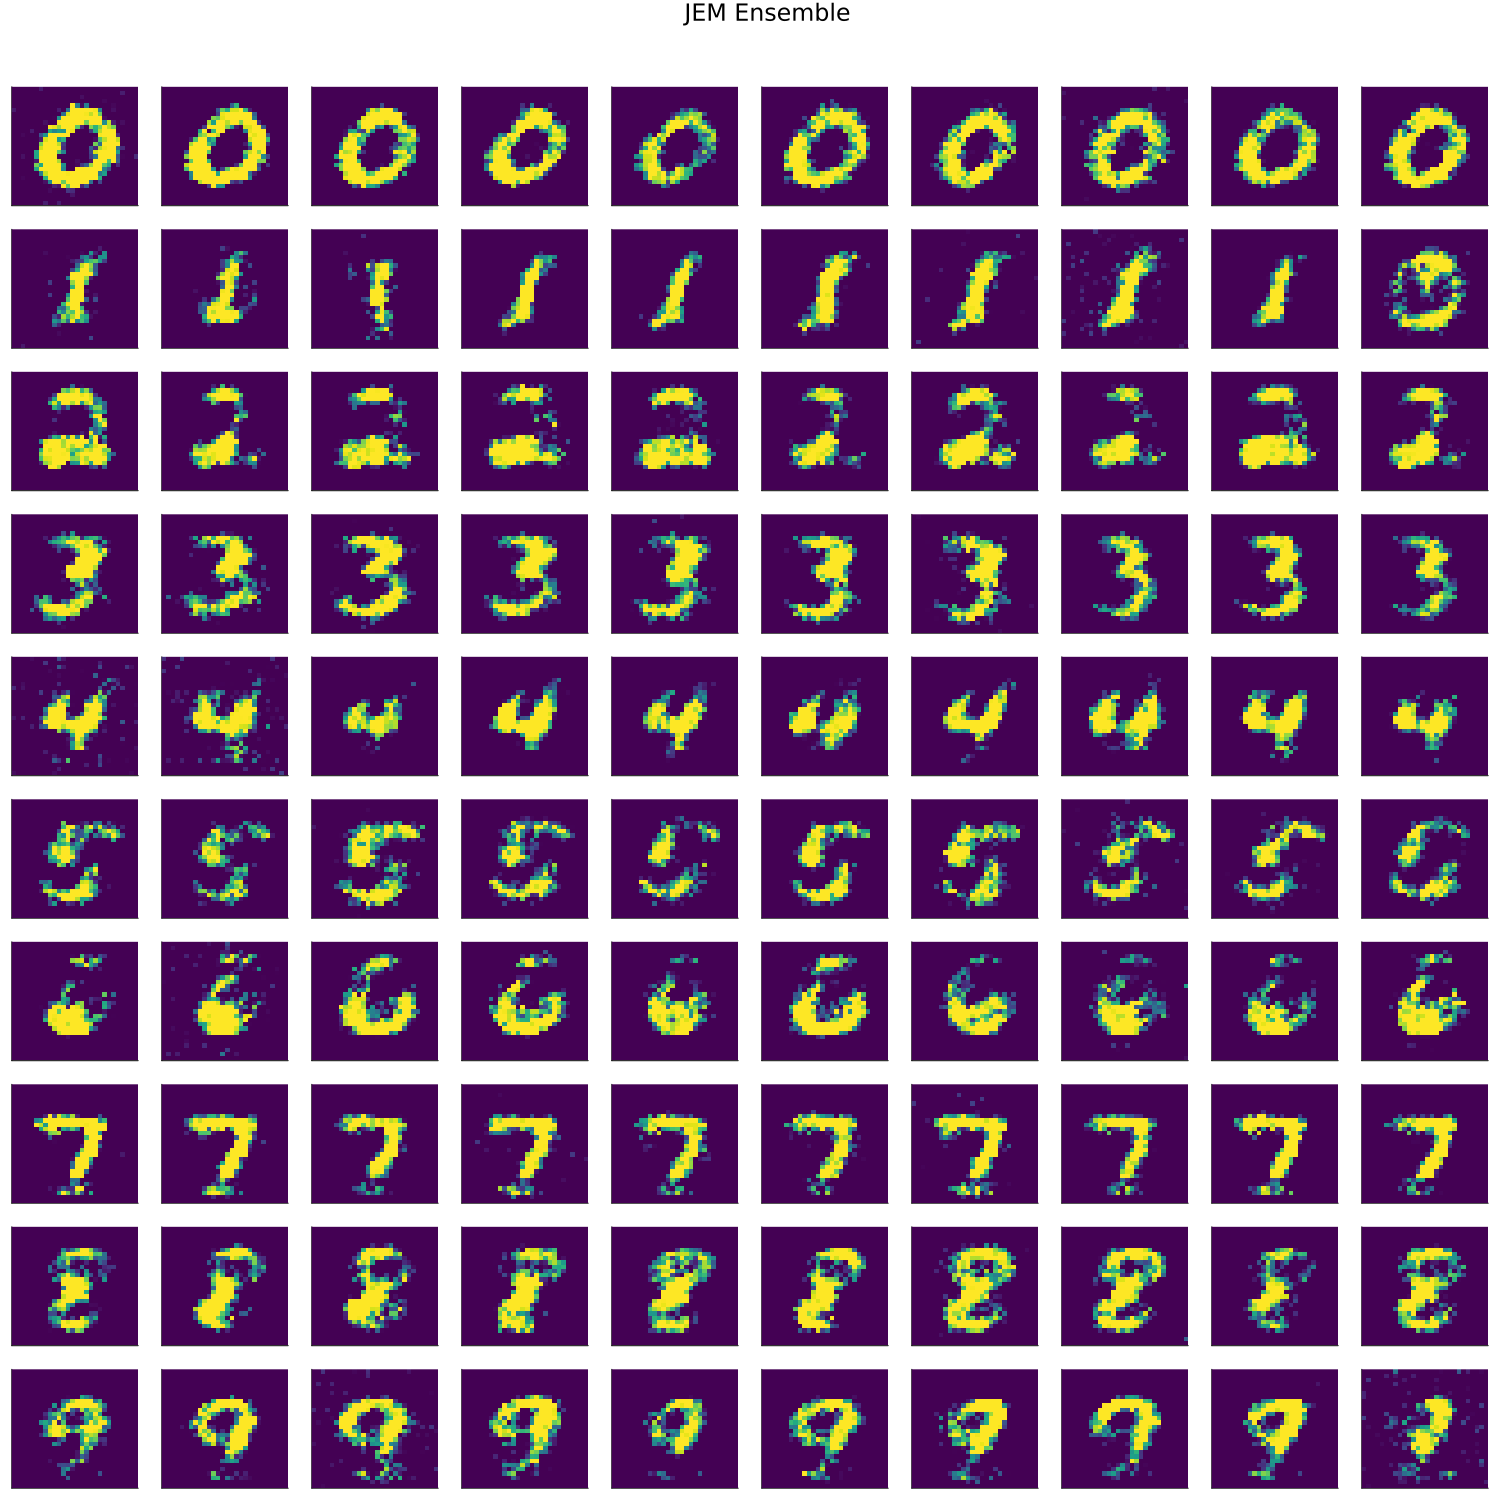
\includegraphics[width=0.75\linewidth]{../artifacts/results/images/mnist_generated_JEM Ensemble.png}
  \caption{Conditionally generated \textit{MNIST} images for our JEM Ensemble.}\label{fig:mnist-gen}
\end{figure}

\begin{figure}
  \centering
  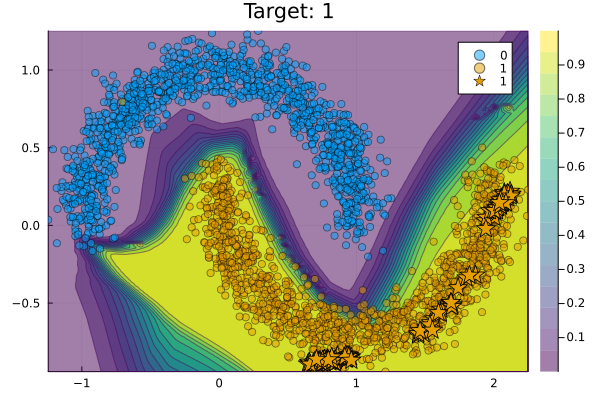
\includegraphics[width=0.5\linewidth]{../artifacts/results/images/moons_generated_JEM.png}
  \caption{Conditionally generated samples (stars) for our \textit{Moons} data using a JEM.}\label{fig:moons-gen}
\end{figure}
\subsubsection{Inference: Quantifying Models' Generative Property}

At inference time, we assume no prior knowledge about the model's generative property. This means that we do not tab into the existing buffer of generated samples for our Joint Energy Models, but instead generate conditional samples from scratch. While we have relied on the default values $\epsilon=2$ and $\sigma=0.01$ also during inference, the number of total SGLD steps was set to $J=500$ in all cases, so significantly higher than during training. For all of our synthetic datasets and models, we generated 50 conditional samples and then formed subsets containing the $n_{E}=25$ lowest-energy samples. While in practice it would be sufficient to do this once for each model and dataset, we have chosen to perform sampling separately for each individual counterfactual in our experiments to account for stochasticity. To help reduce the computational burden for our real-world datasets we have generated only 10 conditional samples each time and used all of them in our counterfactual search. Using more samples, as we originally did, had no substantial impact on our results.

\subsection{Conformal Prediction}\label{app:cp}

In this Appendix~\ref{app:cp} we provide some more background on CP and explain in some more detail how we have used recent advances in Conformal Training for our purposes.

\subsubsection{Background on CP}

Intuitively, CP works under the premise of turning heuristic notions of uncertainty into rigorous uncertainty estimates by repeatedly sifting through the data. It can be used to generate prediction intervals for regression models and prediction sets for classification models. Since the literature on CE and AR is typically concerned with classification problems, we focus on the latter. A particular variant of CP called Split Conformal Prediction (SCP) is well-suited for our purposes, because it imposes only minimal restrictions on model training. 

Specifically, SCP involves splitting the data $\mathcal{D}_n=\{(\mathbf{x}_i,\mathbf{y}_i)\}_{i=1,...,n}$ into a proper training set $\mathcal{D}_{\text{train}}$ and a calibration set $\mathcal{D}_{\text{cal}}$. The former is used to train the classifier in any conventional fashion. The latter is then used to compute so-called nonconformity scores: $\mathcal{S}=\{s(\mathbf{x}_i,\mathbf{y}_i)\}_{i \in \mathcal{D}_{\text{cal}}}$ where $s: (\mathcal{X},\mathcal{Y}) \mapsto \mathbb{R}$ is referred to as \textit{score function}. In the context of classification, a common choice for the score function is just $s_i=1-M_{\theta}(\mathbf{x}_i)[\mathbf{y}_i]$, that is one minus the softmax output corresponding to the observed label $\mathbf{y}_i$~\citep{angelopoulos2021gentle}. 

Finally, classification sets are formed as follows,

\begin{equation}\label{eq:scp}
  \begin{aligned}
    C_{\theta}(\mathbf{x}_i;\alpha)=\{\mathbf{y}: s(\mathbf{x}_i,\mathbf{y}) \le \hat{q}\}
  \end{aligned}
\end{equation}

where $\hat{q}$ denotes the $(1-\alpha)$-quantile of $\mathcal{S}$ and $\alpha$ is a predetermined error rate. As the size of the calibration set increases, the probability that the classification set $C(\mathbf{x}_{\text{test}})$ for a newly arrived sample $\mathbf{x}_{\text{test}}$ does not cover the true test label $\mathbf{y}_{\text{test}}$ approaches $\alpha$~\citep{angelopoulos2021gentle}. 

Observe from Equation~\ref{eq:scp} that Conformal Prediction works on an instance-level basis, much like CE are local. The prediction set for an individual instance $\mathbf{x}_i$ depends only on the characteristics of that sample and the specified error rate. Intuitively, the set is more likely to include multiple labels for samples that are difficult to classify, so the set size is indicative of predictive uncertainty. To see why this effect is exacerbated by small choices for $\alpha$ consider the case of $\alpha=0$, which requires that the true label is covered by the prediction set with probability equal to 1.

\subsubsection{Differentiability}\label{app:cp-diff}

The fact that conformal classifiers produce set-valued predictions introduces a challenge: it is not immediately obvious how to use such classifiers in the context of gradient-based counterfactual search. Put differently, it is not clear how to use prediction sets in Equation~\ref{eq:general}. Fortunately, \citet{stutz2022learning} have recently proposed a framework for Conformal Training that also hinges on differentiability. Specifically, they show how Stochastic Gradient Descent can be used to train classifiers not only for the discriminative task but also for additional objectives related to Conformal Prediction. One such objective is \textit{efficiency}: for a given target error rate $\alpha$, the efficiency of a conformal classifier improves as its average prediction set size decreases. To this end, the authors introduce a smooth set size penalty defined in Equation~\ref{eq:setsize} in the body of this paper. Formally, it is defined as $C_{\theta,\mathbf{y}}(\mathbf{x}_i;\alpha):=\sigma\left((s(\mathbf{x}_i,\mathbf{y})-\alpha) T^{-1}\right)$ for $\mathbf{y}\in\mathcal{Y}$, where $\sigma$ is the sigmoid function and $T$ is a hyper-parameter used for temperature scaling~\citep{stutz2022learning}.

In addition to the smooth set size penalty,~\citet{stutz2022learning} also propose a configurable classification loss function, that can be used to enforce coverage. For \textit{MNIST} data, we found that using this function generally improved the visual quality of the generated counterfactuals, so we used it in our experiments involving real-world data. For the synthetic dataset, visual inspection of the counterfactuals showed that using the configurable loss function sometimes led to overshooting: counterfactuals would end up deep inside the target domain but far away from the observed samples. For this reason, we instead relied on standard cross-entropy loss for our synthetic datasets. As we have noted in the body of the paper, more experimental work is certainly needed in this context. Figure~\ref{fig:cp-diff} shows the prediction set size (left), smooth set size loss (centre) and configurable classification loss (right) for a \textit{JEM} trained on our \textit{Linearly Separable} data.

\begin{figure}
  \centering
  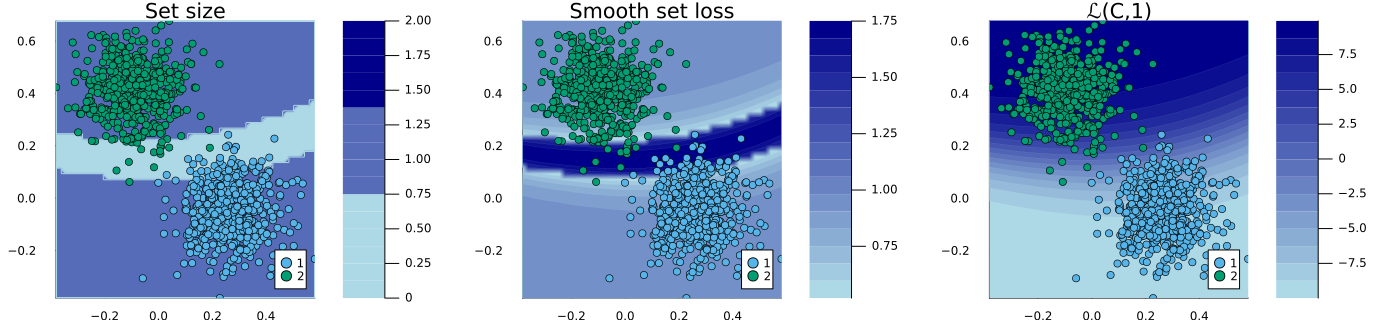
\includegraphics[width=1.0\linewidth]{../artifacts/results/images/poc_set_size.png}
  \caption{Prediction set size (left), smooth set size loss (centre) and configurable classification loss (right) for a JEM trained on our \textit{Linearly Separable} data.}\label{fig:cp-diff}
\end{figure}

\subsection{\textit{ECCCo}}\label{app:eccco}

In this section, we explain \textit{ECCCo} in some more detail, briefly discuss convergence conditions for counterfactual explanations and provide details concerning the actual implementation of our framework in \texttt{Julia}.  

\subsubsection{Deriving the search objective} 

The counterfactual search objective for \textit{ECCCo} was introduced in Equation~\ref{eq:eccco} in the body of the paper. We restate this equation here for reference:

\begin{equation} \label{eq:eccco-app}
  \begin{aligned}
  \mathbf{Z}^\prime &= \arg \min_{\mathbf{Z}^\prime \in \mathcal{Z}^L} \{  {\text{yloss}(M_{\theta}(f(\mathbf{Z}^\prime)),\mathbf{y}^+)}+ \lambda_{1} {\text{dist}(f(\mathbf{Z}^\prime),\mathbf{x}) } \\
  &+ \lambda_2 \mathcal{E}_{\theta}(\mathbf{Z}^\prime,\widehat{\mathbf{X}}_{\theta,\mathbf{y}^+}) + \lambda_3 \Omega(C_{\theta}(f(\mathbf{Z}^\prime);\alpha)) \} 
  \end{aligned} 
\end{equation}

We can make the connection to energy-based modeling more explicit by restating the counterfactual search objective in terms $L_{\text{JEM}}(\theta)$, which we defined in Equation~\ref{eq:jem-loss}. In particular, consider the following counterfactual search objective,

\begin{equation} \label{eq:eccco-jem}
  \begin{aligned}
  \mathbf{Z}^\prime &= \arg \min_{\mathbf{Z}^\prime \in \mathcal{Z}^L} \{  {L_{\text{JEM}}(\theta;M_{\theta}(f(\mathbf{Z}^\prime)),\mathbf{y}^+)}+ \lambda_{1} {\text{dist}(f(\mathbf{Z}^\prime),\mathbf{x}) }  + \lambda_3 \Omega(C_{\theta}(f(\mathbf{Z}^\prime);\alpha)) \} 
  \end{aligned} 
\end{equation}

where we have simply used the JEM loss function as $\text{yloss}(M_{\theta}(f(\mathbf{Z}^\prime)),\mathbf{y}^+)$.

Now note that aside from the additional penalties in Equation~\ref{eq:eccco-app}, the only key difference between our counterfactual search objective and the joint-energy training objective is the parameter that is being optimized. In joint-energy training we optimize the objective with respect to the network weights $\theta$. Recall that $\mathcal{E}_{\theta}(\mathbf{x}|\mathbf{y})=\mu_{\theta}(\mathbf{x})[\mathbf{y}]$. Then the partial gradient with respect to the generative loss component of $L_{\text{JEM}}(\theta)$ can be expressed as follows:

\begin{equation}\label{eq:jem-grad}
  \begin{aligned}
    \nabla_{\theta}L_{\text{gen}}(\theta) &= \nabla_{\theta}\mu_{\theta}(\mathbf{x})[\mathbf{y}]- \nabla_{\theta}\mu_{\theta}(\hat{\mathbf{x}}_{J})[\mathbf{y}]
  \end{aligned}
\end{equation}

During the counterfactual search, we take the network parameters as fixed and instead optimize with respect to the counterfactual itself\footnote{Here we omit the notion of a latent search space to make the comparison easier.},

\begin{equation}\label{eq:ce-grad}
  \begin{aligned}
    \nabla_{\mathbf{x}}L_{\text{gen}}(\theta) &= \nabla_{\mathbf{x}}\mu_{\theta}(\mathbf{x})[\mathbf{y}^+]- \nabla_{\mathbf{x}}\mu_{\theta}(\hat{\mathbf{x}}_{J})[\mathbf{y}^+]=\nabla_{\mathbf{x}}\mu_{\theta}(\mathbf{x})[\mathbf{y}^+]=\nabla_{\mathbf{x}}\mathcal{E}_{\theta}(\mathbf{x}|\mathbf{y}^+)
  \end{aligned}
\end{equation}

where the second term is equal to zero because $\mu_{\theta}(\hat{\mathbf{x}}_{J})[\mathbf{y}]$ is invariant with respect to $\mathbf{x}$. Since this term has zero gradients, we can remove it from the loss function altogether. For the regularization loss component of $L_{\text{JEM}}(\theta)$ we can proceed analogously such that we can rewrite Equation~\ref{eq:eccco-jem} as follows:

\begin{equation} \label{eq:eccco-jem-2}
  \begin{aligned}
  \mathbf{Z}^\prime =& \arg \min_{\mathbf{Z}^\prime \in \mathcal{Z}^L} \{  {\text{yloss}(M_{\theta}(f(\mathbf{Z}^\prime)),\mathbf{y}^+) + \mathcal{E}_{\theta}(f(\mathbf{Z}^\prime)|\mathbf{y}^+) + || \mathcal{E}_{\theta}(f(\mathbf{Z}^\prime)|\mathbf{y}^+) ||_2^2} \\ &+ \lambda_{1} {\text{dist}(f(\mathbf{Z}^\prime),\mathbf{x}) }  + \lambda_3 \Omega(C_{\theta}(f(\mathbf{Z}^\prime);\alpha)) \} 
  \end{aligned} 
\end{equation}

Now we notice that Equation~\ref{eq:eccco-jem-2} is equivalent to Equation~\ref{eq:eccco-app} for $\lambda_2=1$. For the sake of simplicity, we omitted the regularization component from Equation~\ref{eq:eccco} in the main text. Intuitively, taking iterative gradient steps according to Equation~\ref{eq:ce-grad} has the effect of constraining the energy of the counterfactual until. The generative property of the underlying model implicitly enters this equation through $\theta$.

\subsubsection{The \textit{ECCCo} algorithm}

Algorithm~\ref{alg:eccco} describes how exactly \textit{ECCCo} works. For the sake of simplicity and without loss of generality, we limit our attention to generating a single counterfactual $\mathbf{x}^\prime=f(\mathbf{z}^\prime)$. The counterfactual state $\mathbf{z}^\prime$ is initialized at the factual $\mathbf{x}$. Other forms of initialization are also suitable but not considered here. For example, one may choose at a small random perturbation to all features~\citep{slack2021counterfactual}. Next, we calibrate the model $M_{\theta}$ through split conformal prediction. Finally, we search counterfactuals through gradient descent where $\mathcal{L}(\mathbf{z}^\prime,\mathbf{y}^+,\widehat{\mathbf{X}}_{\theta,\mathbf{y}^+}; \Lambda, \alpha)$ denotes our loss function defined in Equation~\ref{eq:eccco}. The search terminates once the convergence criterium is met or the maximum number of iterations $T$ has been exhausted. Note that the choice of convergence criterium has important implications on the final counterfactual which we explain below.

\begin{algorithm*}[h]
  \caption{The \textit{ECCCo} generator}\label{alg:eccco}
  \begin{algorithmic}[1]
    \Require $\mathbf{x}, \mathbf{y}^+, M_{\theta}, \Lambda=[\lambda_1,\lambda_2,\lambda_3], \alpha, \mathcal{D}, T$ where $M_{\theta}(\mathbf{x})\neq\mathbf{y}^+$
    \Ensure $\mathbf{x}^\prime$
    \State Initialize $\mathbf{z}^\prime \gets \mathbf{x}$ 
    \State Run \textit{SCP} for $M_{\theta}$ using $\mathcal{D}$ \Comment{Calibrate model through split conformal prediction.}
    \State Initialize $t \gets 0$
    \While{\textit{not converged} or $t < T$} \Comment{For convergence conditions see below.}
    \State $\mathbf{z}^\prime \gets \mathbf{z}^\prime - \eta \nabla_{\mathbf{z}^\prime} \mathcal{L}(\mathbf{z}^\prime,\mathbf{y}^+,\widehat{\mathbf{X}}_{\theta,\mathbf{y}^+}; \Lambda, \alpha)$ \Comment{Take gradient step of size $\eta$.}
    \State $t \gets t+1$
    \EndWhile
    \State $\mathbf{x}^\prime \gets \mathbf{z}^\prime$ \Comment{Map back to feature space.}
  \end{algorithmic}
\end{algorithm*}

\subsubsection{The \textit{ECCCo+} algorithm}

Algorithm~\ref{alg:eccco-plus} describes how exactly \textit{ECCCo+} works. The only difference to \textit{ECCCo} is that we encode and decode features using PCA.

\begin{algorithm*}[h]
  \caption{The \textit{ECCCo+} generator}\label{alg:eccco-plus}
  \begin{algorithmic}[1]
    \Require $\mathbf{x}, \mathbf{y}^+, M_{\theta}, f, \Lambda=[\lambda_1,\lambda_2,\lambda_3], \alpha, \mathcal{D}, T$ where $M_{\theta}(\mathbf{x})\neq\mathbf{y}^+$
    \Ensure $\mathbf{x}^\prime$
    \State Initialize $\mathbf{z}^\prime \gets f^{-1}(\mathbf{x})$ \Comment{Map to counterfactual state space.}
    \State Run \textit{SCP} for $M_{\theta}$ using $\mathcal{D}$ \Comment{Calibrate model through split conformal prediction.}
    \State Initialize $t \gets 0$
    \While{\textit{not converged} or $t < T$} \Comment{For convergence conditions see below.}
    \State $\mathbf{z}^\prime \gets \mathbf{z}^\prime - \eta \nabla_{\mathbf{z}^\prime} \mathcal{L}(\mathbf{z}^\prime,\mathbf{y}^+,\widehat{\mathbf{X}}_{\theta,\mathbf{y}^+}; \Lambda, \alpha)$ \Comment{Take gradient step of size $\eta$.}
    \State $t \gets t+1$
    \EndWhile
    \State $\mathbf{x}^\prime \gets f(\mathbf{z}^\prime)$ \Comment{Map back to feature space.}
  \end{algorithmic}
\end{algorithm*}

\subsubsection{The \textit{ECCCo-L1} algorithm}

Algorithm~\ref{alg:eccco} describes how exactly \textit{ECCCo} works. For the sake of simplicity and without loss of generality, we limit our attention to generating a single counterfactual $\mathbf{x}^\prime=f(\mathbf{z}^\prime)$. The counterfactual state $\mathbf{z}^\prime$ is initialized by passing the factual $\mathbf{x}$ through a simple feature transformer $f^{-1}$. Next, we generate $n_{\mathcal{B}}$ conditional samples $\hat{\mathbf{x}}_{\theta,\mathbf{y}^+}$ using SGLD (Equation~\ref{eq:sgld}) and store the $n_E$ instances with the lowest energy. We then calibrate the model $M_{\theta}$ through split conformal prediction. Finally, we search counterfactuals through gradient descent where $\mathcal{L}(\mathbf{z}^\prime,\mathbf{y}^+,\widehat{\mathbf{X}}_{\theta,\mathbf{y}^+}; \Lambda, \alpha)$ denotes our loss function defined in Equation~\ref{eq:eccco}. The search terminates once the convergence criterium is met or the maximum number of iterations $T$ has been exhausted. Note that the choice of convergence criterium has important implications on the final counterfactual which we explain in Appendix~\ref{app:eccco}.

\begin{algorithm*}[h]
  \caption{The \textit{ECCCo-L1} generator}\label{alg:eccco-l1}
  \begin{algorithmic}[1]
    \Require $\mathbf{x}, \mathbf{y}^+, M_{\theta}, f, \Lambda=[\lambda_1,\lambda_2,\lambda_3], \alpha, \mathcal{D}, T, \eta, n_{\mathcal{B}}, n_E$ where $M_{\theta}(\mathbf{x})\neq\mathbf{y}^+$
    \Ensure $\mathbf{x}^\prime$
    \State Initialize $\mathbf{z}^\prime \gets f^{-1}(\mathbf{x})$ \Comment{Map to counterfactual state space.}
    \State Generate $\left\{\hat{\mathbf{x}}_{\theta,\mathbf{y}^+}\right\}_{n_{\mathcal{B}}} \gets p_{\theta}(\mathbf{x}_{\mathbf{y}^+})$ \Comment{Generate $n_{\mathcal{B}}$ samples using SGLD (Equation~\ref{eq:sgld}).}
    \State Store $\widehat{\mathbf{X}}_{\theta,\mathbf{y}^+} \gets \left\{\hat{\mathbf{x}}_{\theta,\mathbf{y}^+}\right\}_{n_{\mathcal{B}}}$ \Comment{Choose $n_E$ lowest-energy samples.}
    \State Run \textit{SCP} for $M_{\theta}$ using $\mathcal{D}$ \Comment{Calibrate model through split conformal prediction.}
    \State Initialize $t \gets 0$
    \While{\textit{not converged} or $t < T$} \Comment{For convergence conditions see Appendix~\ref{app:eccco}.}
    \State $\mathbf{z}^\prime \gets \mathbf{z}^\prime - \eta \nabla_{\mathbf{z}^\prime} \mathcal{L}(\mathbf{z}^\prime,\mathbf{y}^+,\widehat{\mathbf{X}}_{\theta,\mathbf{y}^+}; \Lambda, \alpha)$ \Comment{Take gradient step of size $\eta$.}
    \State $t \gets t+1$
    \EndWhile
    \State $\mathbf{x}^\prime \gets f(\mathbf{z}^\prime)$ \Comment{Map back to feature space.}
  \end{algorithmic}
\end{algorithm*}

\subsubsection{A Note on Convergence}\label{convergence}

Convergence is not typically discussed much in the context of CE, even though it has important implications on outcomes. One intuitive way to specify convergence is in terms of threshold probabilities: once the predicted probability $p(\mathbf{y}^+|\mathbf{x}^{\prime})$ exceeds some user-defined threshold $\gamma$ such that the counterfactual is valid, we could consider the search to have converged. In the binary case, for example, convergence could be defined as $p(\mathbf{y}^+|\mathbf{x}^{\prime})>0.5$ in this sense. Note, however, how this can be expected to yield counterfactuals in the proximity of the decision boundary, a region characterized by high aleatoric uncertainty. In other words, counterfactuals generated in this way would generally not be plausible. To avoid this from happening, we specify convergence in terms of gradients approaching zero for all our experiments and all of our generators. This is allows us to get a cleaner read on how the different counterfactual search objectives affect counterfactual outcomes. 

\subsubsection{\texttt{ECCCo.jl}}

The core part of our code base is integrated into a larger ecosystem of \texttt{Julia} packages that we are actively developing and maintaining. To avoid compromising the double-blind review process, we only provide a link to an anonymized repository at this stage: \url{https://anonymous.4open.science/r/ECCCo-1252/README.md}. 

\subsection{Experimental Setup}\label{app:setup}

Table~\ref{tab:params} provides an overview of all parameters related to our experiments. The \textit{GMSC} data were randomly undersampled for balancing purposes and all features were standardized. \textit{MNIST} data was also randomly undersampled for reasons outlined below. Pixel values were preprocessed to fall in the range of $[-1,1]$ and a small Gaussian noise component ($\sigma=0.03$) was added to training samples following common practice in the EBM literature. All of our models were trained through mini-batch training using the Adam optimiser (\citet{kingma2014adam}). Table~\ref{tab:perf} shows standard evaluation metrics measuring the predictive performance of our different models grouped by dataset. These measures were computed on test data. 

Table~\ref{tab:genparams} summarises our hyperparameter choices for the counterfactual generators where $\eta$ denotes the learning rate used for Stochastic Gradient Descent (SGD) and $\lambda_1$, $\lambda_2$, $\lambda_3$ represent the chosen penalty strengths (Equations~\ref{eq:general} and~\ref{eq:eccco}). Here $\lambda_1$ also refers to the chosen penalty for the distance from factual values that applies to both \textit{Wachter} and \textit{REVISE}, but not \textit{Schut} which is penalty-free. \textit{Schut} is also the only generator that uses JSMA instead of SGD for optimization.

\import{contents/}{table_params.tex}

\import{contents/}{table_perf.tex}

\import{contents/}{table_gen_params.tex}

\subsection{Compute}

To enable others to easily replicate our experiments, we have chosen to work with small neural network architectures and randomly undersampled the \textit{MNIST} dataset (maintaining class balance). All of our final benchmarks could then be run locally on a personal machine, but grid searches and the sheer number of datasets required us to move to high-performance computing clusters to conduct our experiments efficiently. 

\subsubsection{Local runs}

The longest runtimes we experienced for model training and counterfactual benchmarking for a single benchmark were on the order of 12-24 hours (\textit{MNIST} data). For the synthetic data, single benchmarks could be completed in less than an hour. We have summarised our system information below:

\textbf{Software}:

\begin{itemize}
  \item System Version: macOS 13.3.1
  \item Kernel Version: Darwin 22.4.0
\end{itemize}

\textbf{Hardware}:

\begin{itemize}
  \item Model Name: MacBook Pro
  \item Model Identifier: MacBookPro16,1
  \item Processor Name: 8-Core Intel Core i9
  \item Processor Speed: 2.3 GHz
  \item Number of Processors: 1
  \item Total Number of Cores: 8
  \item L2 Cache (per Core): 256 KB
  \item L3 Cache: 16 MB
  \item Hyper-Threading Technology: Enabled
  \item Memory: 32 GB
\end{itemize}

\subsubsection{HPC}

We used two large clusters, which we do not cite or mention by name at this point to not interfer with the double-blind review process. All of our grid searches were multi-processed on 100 CPUs at 4-8GB or memory each. 

\subsection{Results}\label{app:results}

Figure~\ref{fig:mnist-eccco} shows examples of counterfactuals for \textit{MNIST} data where the underlying model is our \textit{JEM Ensemble}. Original images are shown on the diagonal and the corresponding counterfactuals are plotted across rows.

\begin{figure}
  \centering
  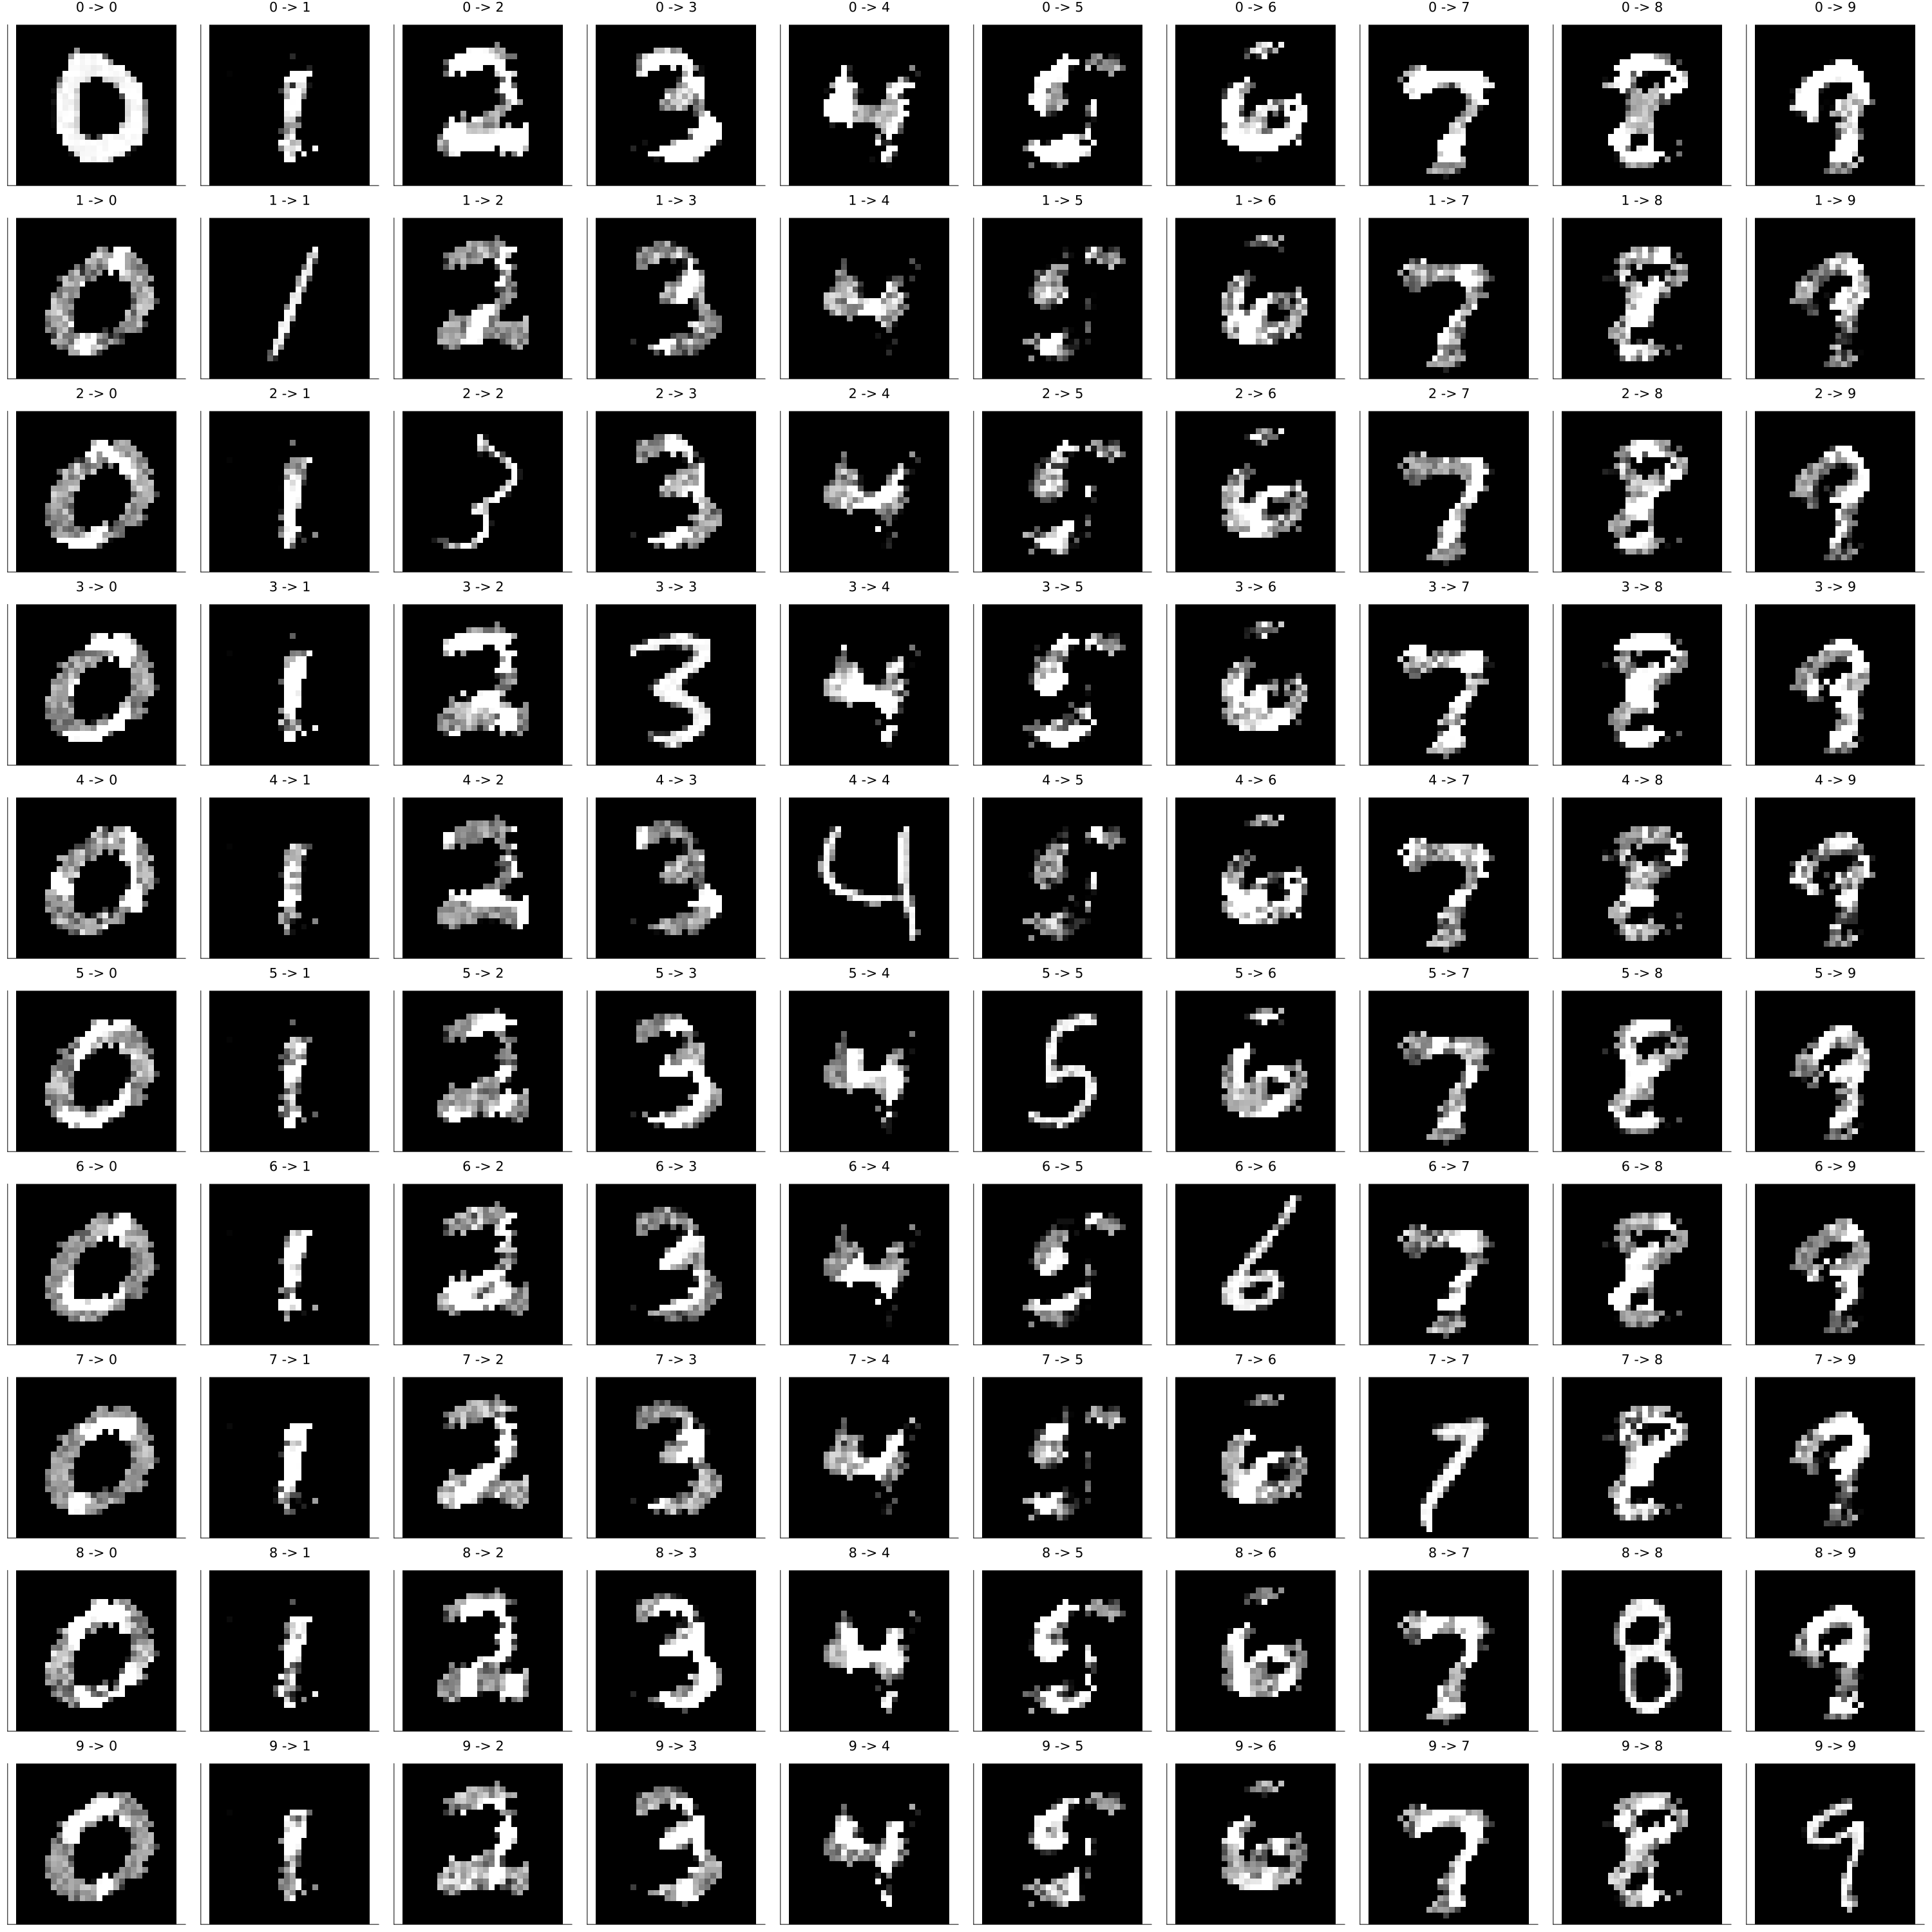
\includegraphics[width=0.9\linewidth]{../artifacts/results/images/mnist_eccco_all_digits.png}
  \caption{Counterfactuals for \textit{MNIST} data and our \textit{JEM Ensemble}. Original images are shown on the diagonal with the corresponding counterfactuals plotted across rows.}\label{fig:mnist-eccco}
\end{figure}

Tables~\ref{tab:results-linearly-separable} to~\ref{tab:results-fashion-mnist} reports all of the evaluation metrics we have computed. Tables~\ref{tab:results-linearly-separable-valid} to~\ref{tab:results-fashion-mnist-valid} reports the same metrics for the subset of valid counterfactuals. The `Unfaithfulness' and `Implausibility' metrics have been discussed extensively in the body of the paper. The `Cost' metric relates to the distance between the factual and the counterfactual and is measured using the L1 Norm. The `Redundancy' metric measures sparsity in is defined as the percentage of features that remain unperturbed (higher is better). The `Uncertainty' metric is just the average value of the smooth set size penalty (Equation~\ref{eq:setsize}). Finally, `Validity' is the percentage of valid counterfactuals. 

\import{contents/}{table-linearly-separable.tex}

\import{contents/}{table-circles.tex}

\import{contents/}{table-moons.tex}

\import{contents/}{table-california-housing.tex}

\import{contents/}{table-gmsc.tex}

\import{contents/}{table-german-credit.tex}

\import{contents/}{table-mnist.tex}

\import{contents/}{table-fashion-mnist.tex}

\import{contents/}{table-linearly-separable-valid.tex}

\import{contents/}{table-circles-valid.tex}

\import{contents/}{table-moons-valid.tex}

\import{contents/}{table-california-housing-valid.tex}

\import{contents/}{table-gmsc-valid.tex}

\import{contents/}{table-german-credit-valid.tex}

\import{contents/}{table-mnist-valid.tex}

\import{contents/}{table-fashion-mnist-valid.tex}